\documentclass[11pt,a4paper]{article}

\usepackage[utf8]{inputenc}
\usepackage[english]{babel}
\usepackage{amsmath,amssymb}
\usepackage{graphicx}
\usepackage{booktabs}
\usepackage{hyperref}
\usepackage{float}
\usepackage{subcaption}
\usepackage[a4paper,margin=2cm]{geometry}
\usepackage{listings}
\usepackage{xcolor}

\lstset{
  basicstyle=\ttfamily\small,
  frame=single,
  breaklines=true,
  language=Python,
  keywordstyle=\color{blue},
  commentstyle=\color{gray},
}

\graphicspath{{../images/}{images/}}

\title{\textbf{APM\_5DS24\_TP -- Deep Learning II}\\[0.3cm]
\large Institut Polytechnique de Paris}
\author{Sergio Magalh\~{a}es Contente}
\date{March 2026}

\begin{document}

\maketitle

\begin{abstract}
This report presents a from-scratch NumPy implementation of Restricted Boltzmann Machines (RBM), Deep Belief Networks (DBN), and Deep Neural Networks (DNN) for handwritten digit classification on MNIST.
We implement unsupervised pre-training via greedy layer-wise RBM training, followed by supervised fine-tuning with backpropagation and a softmax classification layer.
A systematic comparison between pre-trained and randomly initialized networks is conducted across three axes: network depth, layer width, and training set size.
As a bonus, we compare five generative models (RBM, DBN, VAE, GAN, DDPM) under a similar parameter budget on MNIST.
\end{abstract}

\newpage
\tableofcontents
\newpage

% ============================================================
\section{Introduction}
% ============================================================

The goal of this project is to implement a pre-trained deep neural network for handwritten digit classification and to evaluate the benefit of unsupervised pre-training compared to random initialization.
The implementation is done entirely in NumPy, following the architecture where an RBM is a building block for a DBN, which in turn provides pre-trained weights for a DNN with an additional softmax classification layer.

We proceed in four stages:
\begin{enumerate}
    \item Implement and validate the RBM on the Binary AlphaDigits dataset (Section~\ref{sec:rbm_alpha});
    \item Extend to DBN and validate on the same dataset (Section~\ref{sec:dbn_alpha});
    \item Build the DNN with pre-training and backpropagation, then conduct a systematic study on MNIST (Section~\ref{sec:dnn_mnist});
    \item Compare generative models as a bonus (Section~\ref{sec:bonus}).
\end{enumerate}

% ============================================================
\section{Implementation}
\label{sec:implementation}
% ============================================================

All core modules are implemented in the \texttt{src/} directory. We describe the key design choices below.

\subsection{RBM (\texttt{src/rbm.py})}

An RBM is represented as a dictionary with fields \texttt{W} (weight matrix, $p \times q$), \texttt{a} (visible biases, $p$), and \texttt{b} (hidden biases, $q$).

\begin{itemize}
    \item \textbf{\texttt{init\_RBM(p, q)}}: Weights are initialized from $\mathcal{N}(0, 0.01)$, biases are set to zero.
    \item \textbf{\texttt{entree\_sortie\_RBM}}: Computes $P(h|v) = \sigma(v W + b)$.
    \item \textbf{\texttt{sortie\_entree\_RBM}}: Computes $P(v|h) = \sigma(h W^\top + a)$.
    \item \textbf{\texttt{train\_RBM}}: Contrastive Divergence-1 (CD-1). For the positive phase gradient, we use the probabilities $P(h|v_0)$ (not samples). For the negative phase, we sample $h_0$, reconstruct $v_1$ as probabilities, then compute $P(h|v_1)$. The reconstruction MSE is reported every 10 epochs.
    \item \textbf{\texttt{generer\_image\_RBM}}: Generates images via Gibbs sampling starting from random binary vectors, alternating between sampling hidden and visible units.
\end{itemize}

\subsection{DBN (\texttt{src/dbn.py})}

A DBN is a list of RBMs trained greedily layer by layer.

\begin{itemize}
    \item \textbf{\texttt{init\_DBN(layer\_sizes)}}: Creates one RBM per consecutive pair of layer sizes. For example, \texttt{[320, 200, 100]} creates two RBMs: $320 \to 200$ and $200 \to 100$.
    \item \textbf{\texttt{train\_DBN}}: Greedy layer-wise training. After training the first RBM, the data is transformed through it (using probabilities, not samples) to produce the input for the next RBM.
    \item \textbf{\texttt{generer\_image\_DBN}}: Gibbs sampling at the top RBM, followed by top-down propagation through all lower layers using $P(v|h)$.
\end{itemize}

\subsection{DNN (\texttt{src/dnn.py})}

A DNN is a DBN augmented with a softmax classification layer.

\begin{itemize}
    \item \textbf{\texttt{init\_DNN(layer\_sizes)}}: For \texttt{[784, 200, 200, 10]}, creates a 2-layer DBN ($784 \to 200 \to 200$) plus a softmax RBM ($200 \to 10$).
    \item \textbf{\texttt{pretrain\_DNN}}: Pre-trains only the hidden layers (excluding the softmax layer) via \texttt{train\_DBN}.
    \item \textbf{\texttt{calcul\_softmax}}: Computes $P(y|h) = \mathrm{softmax}(hW + b)$ with numerical stability (subtracting the max logit).
    \item \textbf{\texttt{entree\_sortie\_reseau}}: Full forward pass. Hidden layers use sigmoid activation; the last layer uses softmax. Returns all intermediate activations (needed for backpropagation).
    \item \textbf{\texttt{retropropagation}}: Backpropagation with cross-entropy loss. The output layer gradient is $\delta = \hat{y} - y$ (softmax + cross-entropy simplification). For hidden layers, the gradient is propagated through the weights \emph{before} updating them, and the sigmoid derivative $h(1-h)$ is applied. As specified, the loss is computed \emph{after} all parameter updates at the end of each epoch via a single full forward pass.
    \item \textbf{\texttt{test\_DNN}}: Computes the classification error rate as the fraction of misclassified samples.
\end{itemize}

\subsection{Data Loading (\texttt{src/utils.py})}

\begin{itemize}
    \item \textbf{\texttt{lire\_alpha\_digit(characters)}}: Loads Binary AlphaDigits from the \texttt{.mat} file. Each character index (0--35) yields 39 binary images of size $20 \times 16 = 320$ pixels.
    \item \textbf{\texttt{load\_mnist()}}: Reads the IDX files, binarizes images at threshold 127, and one-hot encodes labels. Returns train and test splits (60,000 / 10,000).
\end{itemize}

% ============================================================
\section{Study on Binary AlphaDigits}
\label{sec:alpha}
% ============================================================

Before tackling MNIST, we validate the RBM and DBN implementations on the Binary AlphaDigits dataset, which contains small ($20 \times 16$) binary images of digits and letters (36 classes, 39 samples each).

% ------------------------------------------------------------
\subsection{RBM Experiments}
\label{sec:rbm_alpha}
% ------------------------------------------------------------

\subsubsection{Original Data}

We train on characters 0, 1, and 2 (117 samples total). Figure~\ref{fig:alpha_originals} shows representative samples.

\begin{figure}[H]
    \centering
    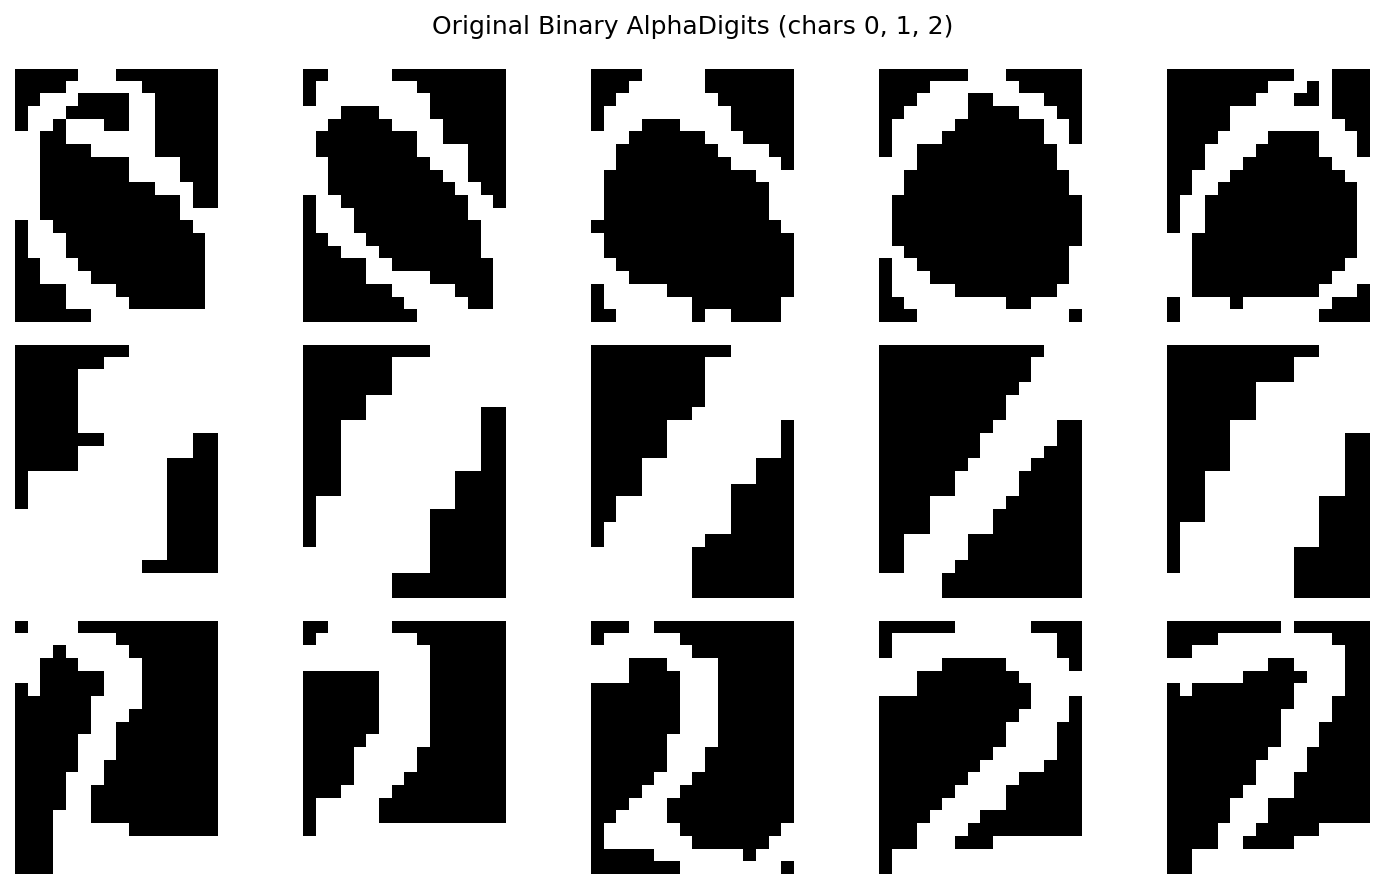
\includegraphics[width=0.8\linewidth]{alpha_originals.png}
    \caption{Original Binary AlphaDigits samples (characters 0, 1, 2).}
    \label{fig:alpha_originals}
\end{figure}

\subsubsection{Effect of the Number of Hidden Units}

We train RBMs with $q \in \{50, 100, 200, 300\}$ hidden units (100 epochs, $\eta = 0.1$, batch size 32) and generate images via 500 Gibbs steps.

\begin{figure}[H]
    \centering
    \begin{subfigure}{0.48\linewidth}
        \centering
        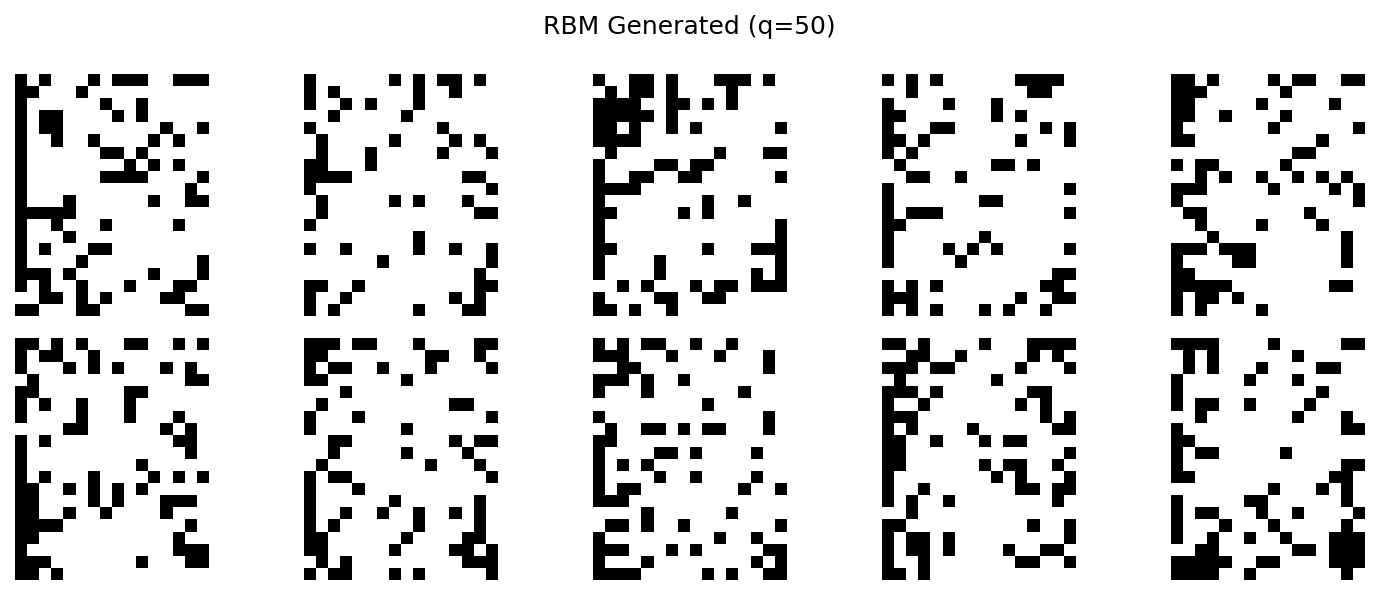
\includegraphics[width=\linewidth]{rbm_alpha_q50.png}
        \caption{$q = 50$}
    \end{subfigure}
    \hfill
    \begin{subfigure}{0.48\linewidth}
        \centering
        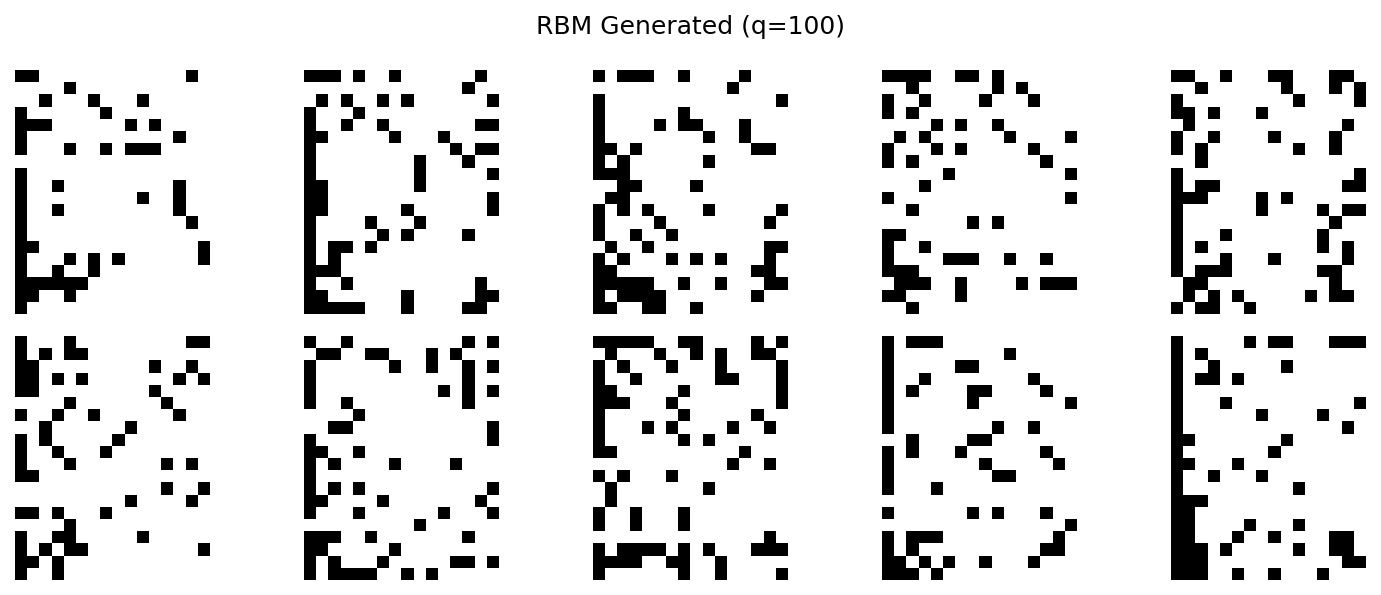
\includegraphics[width=\linewidth]{rbm_alpha_q100.png}
        \caption{$q = 100$}
    \end{subfigure}

    \vspace{0.3cm}

    \begin{subfigure}{0.48\linewidth}
        \centering
        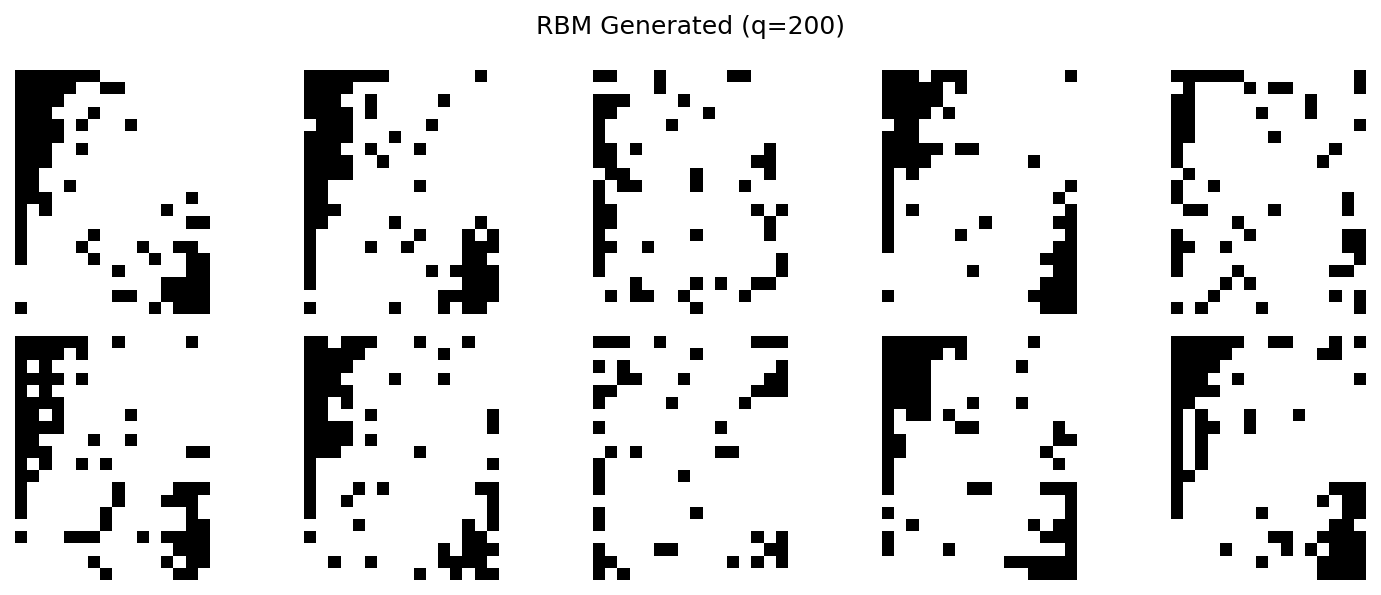
\includegraphics[width=\linewidth]{rbm_alpha_q200.png}
        \caption{$q = 200$}
    \end{subfigure}
    \hfill
    \begin{subfigure}{0.48\linewidth}
        \centering
        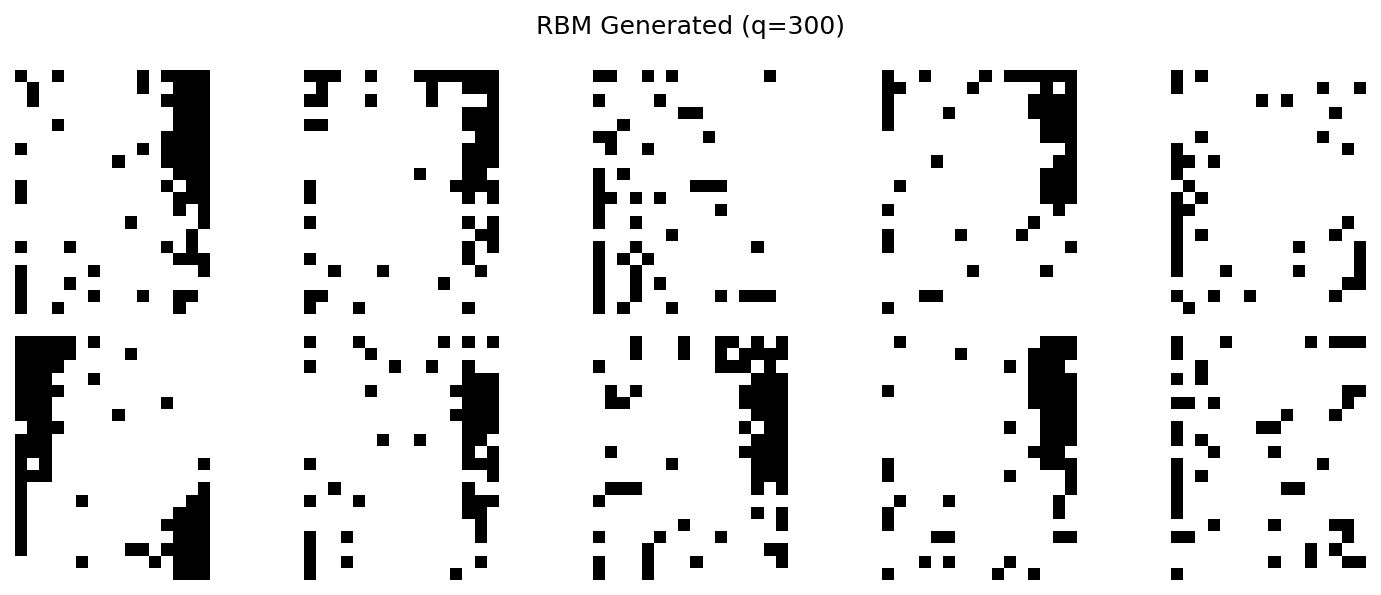
\includegraphics[width=\linewidth]{rbm_alpha_q300.png}
        \caption{$q = 300$}
    \end{subfigure}
    \caption{RBM-generated images as a function of the number of hidden units $q$.}
    \label{fig:rbm_q}
\end{figure}

With $q = 50$, the generated images are very noisy with almost no discernible structure, indicating insufficient capacity to capture the data distribution. At $q = 100$, some local structure begins to emerge --- contiguous black regions and edges become visible, though the images remain noisy. With $q = 200$ and $q = 300$, the generated images show clearer block structures reminiscent of the training characters, with recognizable vertical and diagonal strokes. The improvement from 200 to 300 is marginal, suggesting that $q = 200$ provides a reasonable trade-off between capacity and the limited training set size (117 samples). Nevertheless, the binary stochastic nature of the Gibbs sampling process inherently produces noisy outputs.

\subsubsection{Effect of Character Diversity}

We fix $q = 200$ and vary the number of characters used for training: 3, 10, and 36 (all alphanumeric characters).

\begin{figure}[H]
    \centering
    \begin{subfigure}{0.32\linewidth}
        \centering
        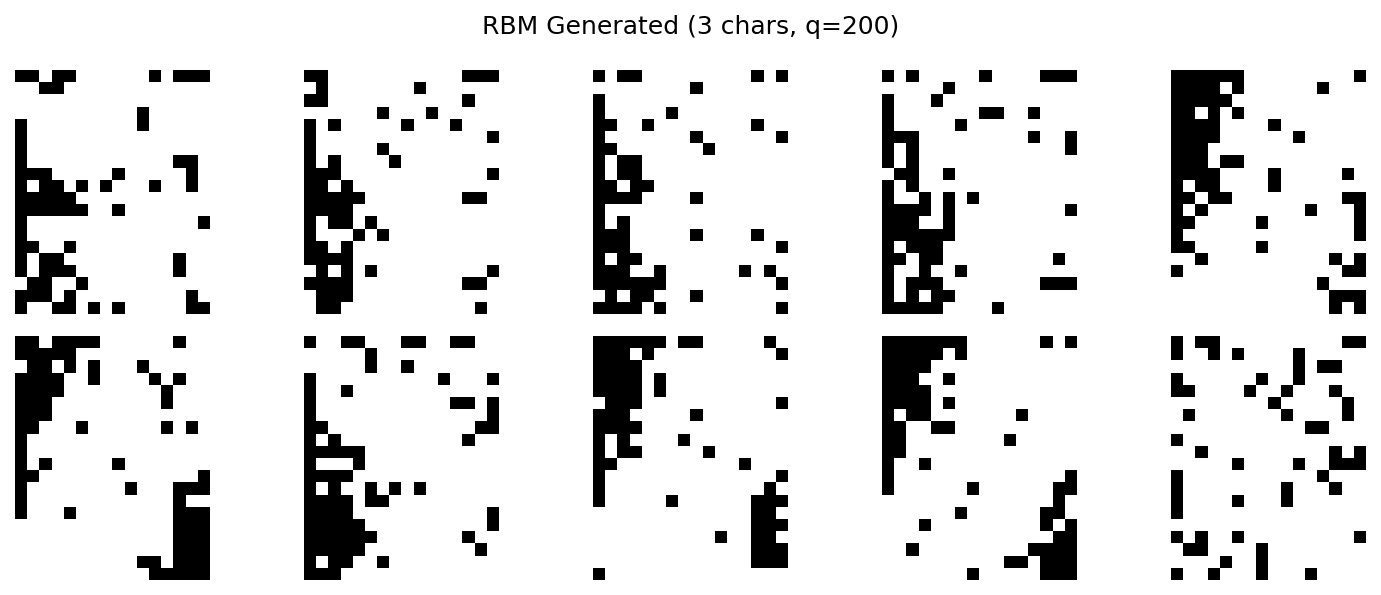
\includegraphics[width=\linewidth]{rbm_alpha_nchars3.png}
        \caption{3 characters}
    \end{subfigure}
    \hfill
    \begin{subfigure}{0.32\linewidth}
        \centering
        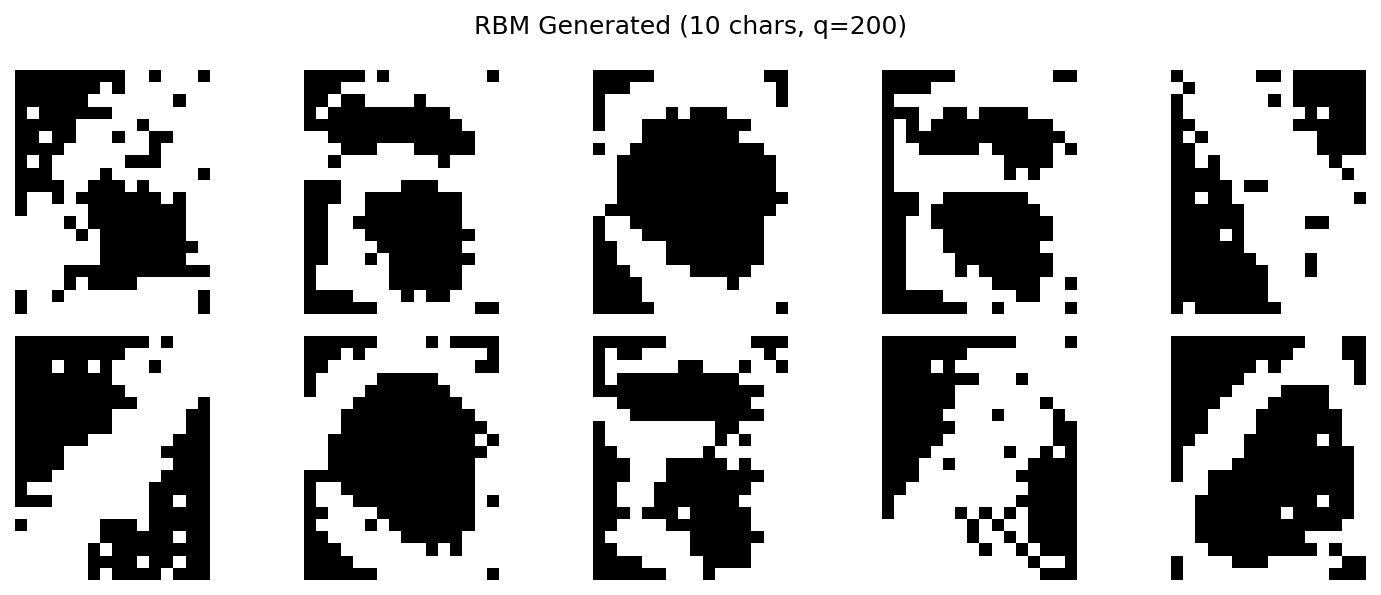
\includegraphics[width=\linewidth]{rbm_alpha_nchars10.png}
        \caption{10 characters}
    \end{subfigure}
    \hfill
    \begin{subfigure}{0.32\linewidth}
        \centering
        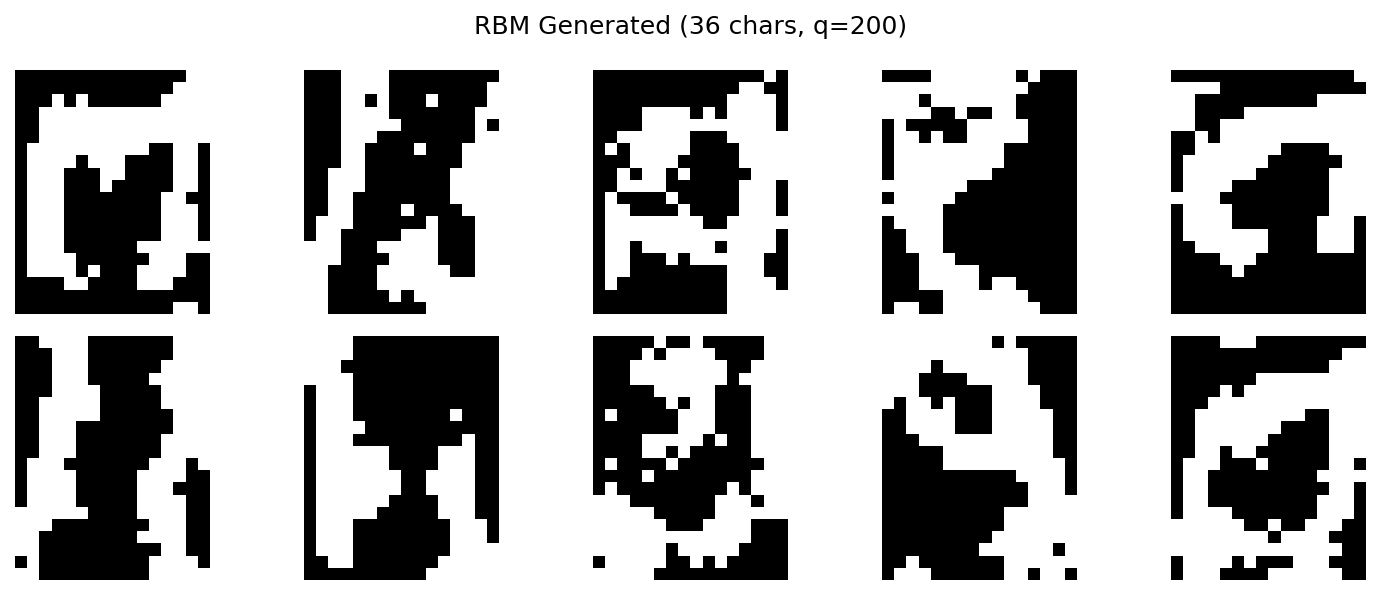
\includegraphics[width=\linewidth]{rbm_alpha_nchars36.png}
        \caption{36 characters}
    \end{subfigure}
    \caption{RBM-generated images as a function of the number of training characters ($q = 200$).}
    \label{fig:rbm_nchars}
\end{figure}

With 3 characters, the generated images capture some structural features of the digits but remain noisy due to the very small training set (117 samples). Interestingly, with 36 characters (1,404 samples), the generated images appear more structured, with clearer character-like shapes. This is because more training data allows the RBM to learn more robust features, even though the distribution is more diverse. The increased data volume compensates for the added complexity, highlighting that RBM quality depends heavily on having sufficient training samples.

% ------------------------------------------------------------
\subsection{DBN Experiments}
\label{sec:dbn_alpha}
% ------------------------------------------------------------

\subsubsection{Effect of Network Depth}

We train DBNs with 1, 2, and 3 hidden layers on characters 0, 1, 2.

\begin{figure}[H]
    \centering
    \begin{subfigure}{0.32\linewidth}
        \centering
        
\includegraphics[width=\linewidth]{dbn_alpha_1layer.png}
        \caption{1 layer: $320 \to 200$}
    \end{subfigure}
    \hfill
    \begin{subfigure}{0.32\linewidth}
        \centering
        
\includegraphics[width=\linewidth]{dbn_alpha_2layers.png}
        \caption{2 layers: $320 \to 200 \to 100$}
    \end{subfigure}
    \hfill
    \begin{subfigure}{0.32\linewidth}
        \centering
        
\includegraphics[width=\linewidth]{dbn_alpha_3layers.png}
        \caption{3 layers: $320 \to 200 \to 100 \to 50$}
    \end{subfigure}
    \caption{DBN-generated images with varying depth.}
    \label{fig:dbn_layers}
\end{figure}

The single-layer DBN (equivalent to an RBM) produces noisy binary images, similar to those from the standalone RBM. The \textbf{2-layer DBN} produces the best results: the top-down propagation through two layers of learned probabilities generates smooth grayscale images with clearly recognizable digit shapes (0s and 2s are distinctly visible). This demonstrates the benefit of hierarchical feature learning --- the first layer captures low-level structure while the second captures higher-level abstractions. The 3-layer DBN, however, produces blurry and less distinct grayscale images. The top RBM operates on only 50 hidden units, which limits the expressiveness of the Gibbs sampling and leads to less informative top-layer representations being propagated downward.

\subsubsection{Effect of Character Diversity on DBN}

We fix the architecture to $320 \to 200 \to 100$ and vary the number of characters.

\begin{figure}[H]
    \centering
    \begin{subfigure}{0.32\linewidth}
        \centering
        
\includegraphics[width=\linewidth]{dbn_alpha_nchars5.png}
        \caption{5 characters}
    \end{subfigure}
    \hfill
    \begin{subfigure}{0.32\linewidth}
        \centering
        
\includegraphics[width=\linewidth]{dbn_alpha_nchars10.png}
        \caption{10 characters}
    \end{subfigure}
    \hfill
    \begin{subfigure}{0.32\linewidth}
        \centering
        
\includegraphics[width=\linewidth]{dbn_alpha_nchars36.png}
        \caption{36 characters}
    \end{subfigure}
    \caption{DBN-generated images as a function of the number of training characters.}
    \label{fig:dbn_nchars}
\end{figure}

The 2-layer DBN produces smooth grayscale images across all diversity levels. With 5 characters, the generated images are the most recognizable. As the number of characters increases to 36, the generated images become more uniform and less class-specific, as the model averages over a wider distribution. Compared to the standalone RBM, the DBN's hierarchical structure and probability-based top-down propagation consistently produce smoother and more recognizable outputs, confirming the benefit of deep generative models even on this small dataset.

% ============================================================
\section{Study on MNIST}
\label{sec:dnn_mnist}
% ============================================================

We now turn to the main study: comparing a pre-trained DNN (unsupervised RBM pre-training + backpropagation) against a randomly initialized DNN (backpropagation only) on MNIST.

\subsection{Experimental Setup}

MNIST images are binarized at threshold 127. For each experiment, two identical DNNs are created. One is pre-trained via greedy layer-wise RBM training (100 epochs per layer), then fine-tuned with backpropagation (200 epochs). The other is trained from random initialization with backpropagation only (200 epochs). Both use learning rate $\eta = 0.1$ and batch size 128. The classification error rate on the test set is reported.

Three experiments are conducted as specified in the assignment:

\subsection{Figure 1: Error Rate vs.\ Number of Hidden Layers}

We fix the number of neurons per hidden layer at 200 and vary the number of hidden layers from 2 to 5. The architecture is $[784, 200, \ldots, 200, 10]$.

\begin{figure}[H]
    \centering
    
\includegraphics[width=0.75\linewidth]{fig1_layers.png}
    \caption{Classification error rate on the test set as a function of the number of hidden layers (200 neurons each). Blue: pre-trained + backpropagation. Red: random initialization + backpropagation.}
    \label{fig:fig1}
\end{figure}

\begin{table}[H]
\centering
\caption{Error rates vs.\ number of hidden layers (200 neurons each).}
\label{tab:fig1}
\begin{tabular}{ccccc}
\toprule
Hidden layers & \multicolumn{2}{c}{Test error (\%)} & \multicolumn{2}{c}{Train error (\%)} \\
\cmidrule(lr){2-3} \cmidrule(lr){4-5}
 & Pre-trained & Random & Pre-trained & Random \\
\midrule
2 & 3.31 & \textbf{2.60} & 0.22 & 0.01 \\
3 & \textbf{2.84} & 3.39 & 0.12 & 0.07 \\
4 & \textbf{2.65} & 7.69 & 0.07 & 5.37 \\
5 & \textbf{2.63} & 88.65 & 0.06 & 88.76 \\
\bottomrule
\end{tabular}
\end{table}

\textbf{Analysis.} With 2 hidden layers, the random network actually slightly outperforms the pre-trained one (2.60\% vs.\ 3.31\%). However, as depth increases, the randomly initialized network degrades dramatically: at 4 layers it reaches 7.69\% error, and at 5 layers the loss remains stuck at $\approx 2.30$ ($= \ln 10$, i.e., random guessing) throughout the entire 200 epochs of training, yielding $\approx 90\%$ error.

This is a textbook demonstration of the \textbf{vanishing gradient problem}: in deep randomly initialized networks, gradients become vanishingly small in the earlier layers, preventing any learning. The loss plateau at $\ln(10)$ confirms the network is outputting uniform softmax probabilities. In contrast, the pre-trained network maintains stable and even slightly improving performance as depth increases (2.65\% at 4 layers), because RBM pre-training places the weights in a favorable region of parameter space where gradients flow effectively.

The key takeaway is that \textbf{pre-training is essential for deep architectures} (more than 2--3 hidden layers). For shallow networks (2 layers), random initialization is competitive. For our best model, we select \textbf{2 hidden layers} since deeper networks do not improve test error despite pre-training.

\subsection{Figure 2: Error Rate vs.\ Number of Neurons per Layer}

We fix the architecture to 2 hidden layers and vary the number of neurons per layer: 100, 300, 500, and 700.

\begin{figure}[H]
    \centering
    
\includegraphics[width=0.75\linewidth]{fig2_neurons.png}
    \caption{Classification error rate vs.\ number of neurons per hidden layer (2 hidden layers). Blue: pre-trained. Red: random init.}
    \label{fig:fig2}
\end{figure}

\begin{table}[H]
\centering
\caption{Error rates vs.\ number of neurons per hidden layer (2 hidden layers).}
\label{tab:fig2}
\begin{tabular}{ccccc}
\toprule
Neurons/layer & \multicolumn{2}{c}{Test error (\%)} & \multicolumn{2}{c}{Train error (\%)} \\
\cmidrule(lr){2-3} \cmidrule(lr){4-5}
 & Pre-trained & Random & Pre-trained & Random \\
\midrule
100 & 4.06 & \textbf{2.86} & 1.16 & 0.01 \\
300 & 3.45 & \textbf{2.69} & 0.06 & 0.02 \\
500 & 3.10 & \textbf{2.67} & 0.01 & 0.04 \\
700 & \textbf{2.48} & 2.67 & 0.00 & 0.07 \\
\bottomrule
\end{tabular}
\end{table}

\textbf{Analysis.} An interesting pattern emerges: for small and medium widths (100--500 neurons), the randomly initialized network actually outperforms the pre-trained one on the test set. However, the pre-trained network improves consistently with more neurons, and at 700 neurons it finally surpasses the random network (2.48\% vs.\ 2.67\%).

This can be explained by examining the train errors: the pre-trained network with 100 neurons has a relatively high train error (1.16\%), suggesting that pre-training may impose a too-rigid initialization for small networks, limiting their flexibility during backpropagation. As width increases, the pre-trained network can better exploit the richer features learned during the unsupervised phase, eventually reaching 0\% train error and the best test error at 700 neurons. The random network plateaus at $\approx 2.67\%$ test error regardless of width beyond 300 neurons. For our best model, \textbf{700 neurons per layer} is optimal.

\subsection{Figure 3: Error Rate vs.\ Number of Training Samples}

We fix the architecture to $[784, 200, 200, 10]$ and vary the number of training samples: 1000, 3000, 7000, 10000, 30000, and 60000.

\begin{figure}[H]
    \centering
    
\includegraphics[width=0.75\linewidth]{fig3_samples.png}
    \caption{Classification error rate vs.\ number of training samples (log scale). Architecture: $[784, 200, 200, 10]$.}
    \label{fig:fig3}
\end{figure}

\begin{table}[H]
\centering
\caption{Error rates vs.\ number of training samples. Architecture: $[784, 200, 200, 10]$.}
\label{tab:fig3}
\begin{tabular}{ccccc}
\toprule
Samples & \multicolumn{2}{c}{Test error (\%)} & \multicolumn{2}{c}{Train error (\%)} \\
\cmidrule(lr){2-3} \cmidrule(lr){4-5}
 & Pre-trained & Random & Pre-trained & Random \\
\midrule
1,000  & \textbf{10.10} & 90.26 & 2.50  & 88.50 \\
3,000  & \textbf{7.01}  & 19.25 & 1.43  & 15.17 \\
7,000  & \textbf{6.20}  & 9.75  & 0.93  & 4.13  \\
10,000 & \textbf{5.69}  & 7.86  & 0.69  & 2.81  \\
60,000 & 3.31           & \textbf{2.60} & 0.22  & 0.01  \\
\bottomrule
\end{tabular}
\end{table}

\textbf{Analysis.} Pre-training provides its greatest advantage in the \textbf{low-data regime}. With only 1,000 training samples, the randomly initialized network is completely stuck at $\approx 90\%$ error (the loss remains at $\ln(10) \approx 2.30$ throughout training, i.e., random guessing), while the pre-trained network achieves 10.10\%. Even with 3,000 samples, the gap is dramatic: 7.01\% vs.\ 19.25\%.

As the dataset grows, the gap narrows. With 10,000 samples, the random network begins to learn effectively (7.86\%), and at 60,000 samples it actually outperforms the pre-trained network (2.60\% vs.\ 3.31\%).

This is consistent with theory: unsupervised pre-training acts as a regularizer by learning the structure of the input distribution. When labeled data is scarce, this prior knowledge is critical --- without it, the randomly initialized network cannot even escape the random-guessing plateau. With abundant labeled data, supervised training alone can discover comparable features, making pre-training unnecessary. For our best model, we use \textbf{all 60,000 training samples}.

\subsection{Best Model Configuration}
\label{sec:best_model}

Based on the three experiments above, the optimal configuration is:

\begin{itemize}
    \item \textbf{Architecture}: $[784, 700, 700, 10]$ --- 2 hidden layers (Fig.~1) with 700 neurons each (Fig.~2)
    \item \textbf{Pre-training}: Yes --- consistently better or equal to random initialization
    \item \textbf{Training data}: All 60,000 samples (Fig.~3)
    \item \textbf{RBM pre-training}: 100 epochs per layer, $\eta = 0.1$
    \item \textbf{Backpropagation}: 200 epochs, $\eta = 0.1$, batch size 128
\end{itemize}

\begin{figure}[H]
    \centering
    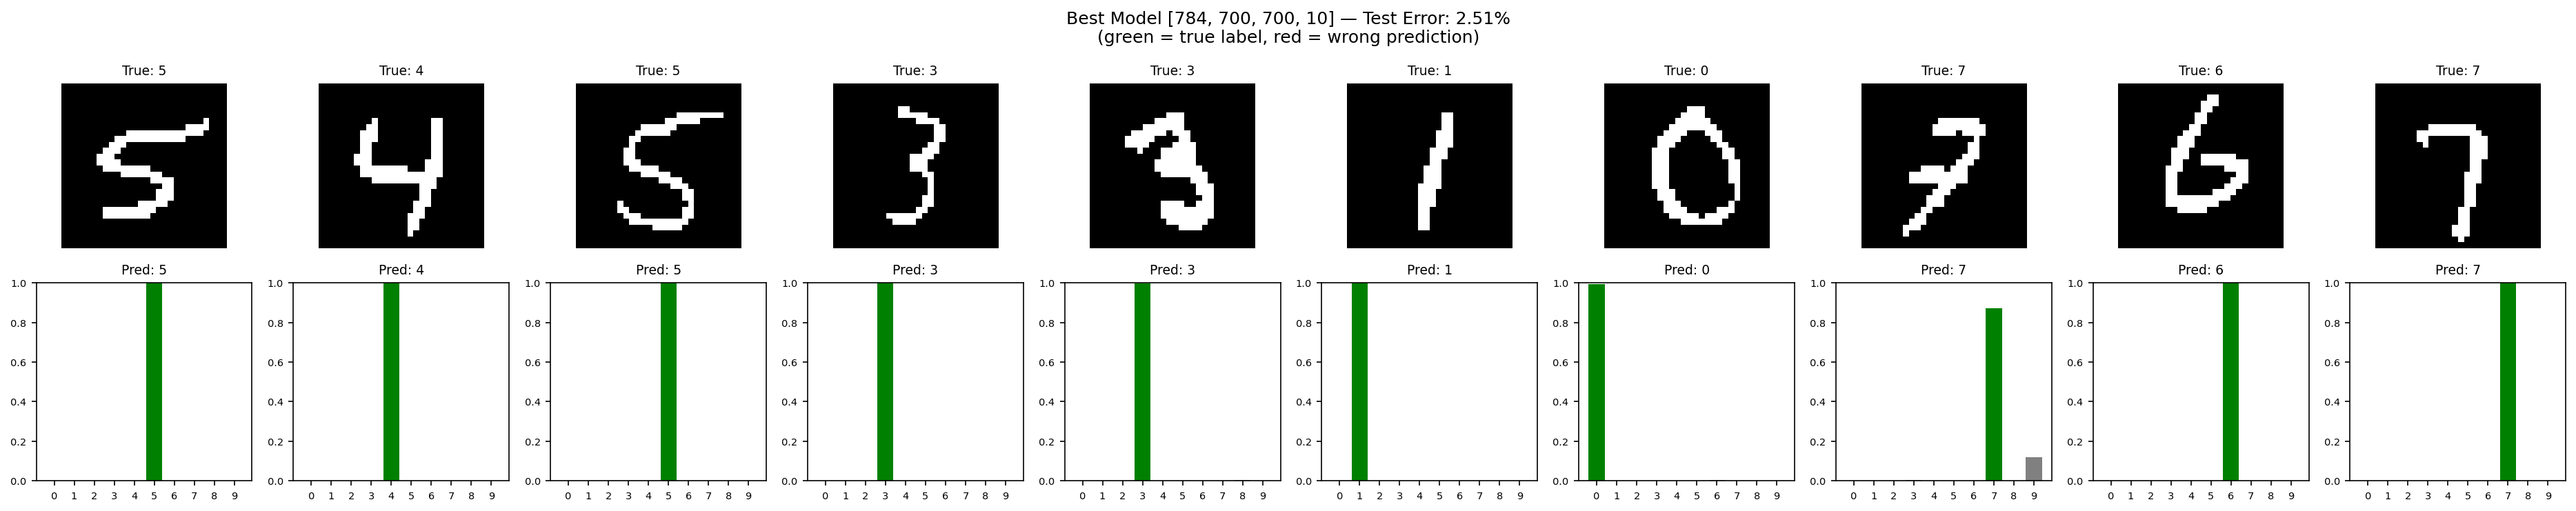
\includegraphics[width=\linewidth]{softmax_best_model.png}
    \caption{Best model predictions on random test samples. Top row: input image with true label. Bottom row: softmax output probabilities (green = true label, red = incorrect prediction).}
    \label{fig:softmax}
\end{figure}

The best model achieves a test error rate of \textbf{2.51\%}. The softmax output probabilities (Figure~\ref{fig:softmax}) show confident and well-calibrated predictions, with the probability mass concentrated almost entirely on the correct class. All 10 randomly selected test samples in the figure are correctly classified with near-certainty.

% ============================================================
\section{Bonus: Generative Models Comparison}
\label{sec:bonus}
% ============================================================

As a bonus, we compare five generative models trained on MNIST with approximately the same number of parameters ($\sim$160k each):

\begin{enumerate}
    \item \textbf{RBM} ($784 \to 200$, $\sim$158k params): 100 epochs of CD-1, generation via 1000 Gibbs steps.
    \item \textbf{DBN} ($784 \to 200 \to 100$, $\sim$178k params): Greedy layer-wise training, generation via Gibbs at top + top-down propagation.
    \item \textbf{VAE} ($784 \to 200 \to 100 \to 20 \to 100 \to 200 \to 784$, $\sim$161k params): Variational autoencoder with reparameterization trick, trained for 200 epochs with Adam.
    \item \textbf{GAN} (Generator: $64 \to 256 \to 512 \to 784$ with BatchNorm; Discriminator: $784 \to 512 \to 256 \to 1$ with Dropout, $\sim$210k params total): Trained for 200 epochs with label smoothing.
    \item \textbf{DDPM} (Denoising Diffusion Probabilistic Model, $\sim$169k params): Simple MLP denoiser with sinusoidal time embeddings, skip connections, GELU activations, $T = 500$ diffusion steps, 200 epochs.
\end{enumerate}

The VAE, GAN, and DDPM are implemented in PyTorch and trained on Google Colab with GPU acceleration. The RBM and DBN use our NumPy implementation. The comparison notebook is self-contained and available at \texttt{notebooks/bonus\_comparison.ipynb}.

\begin{figure}[H]
    \centering
    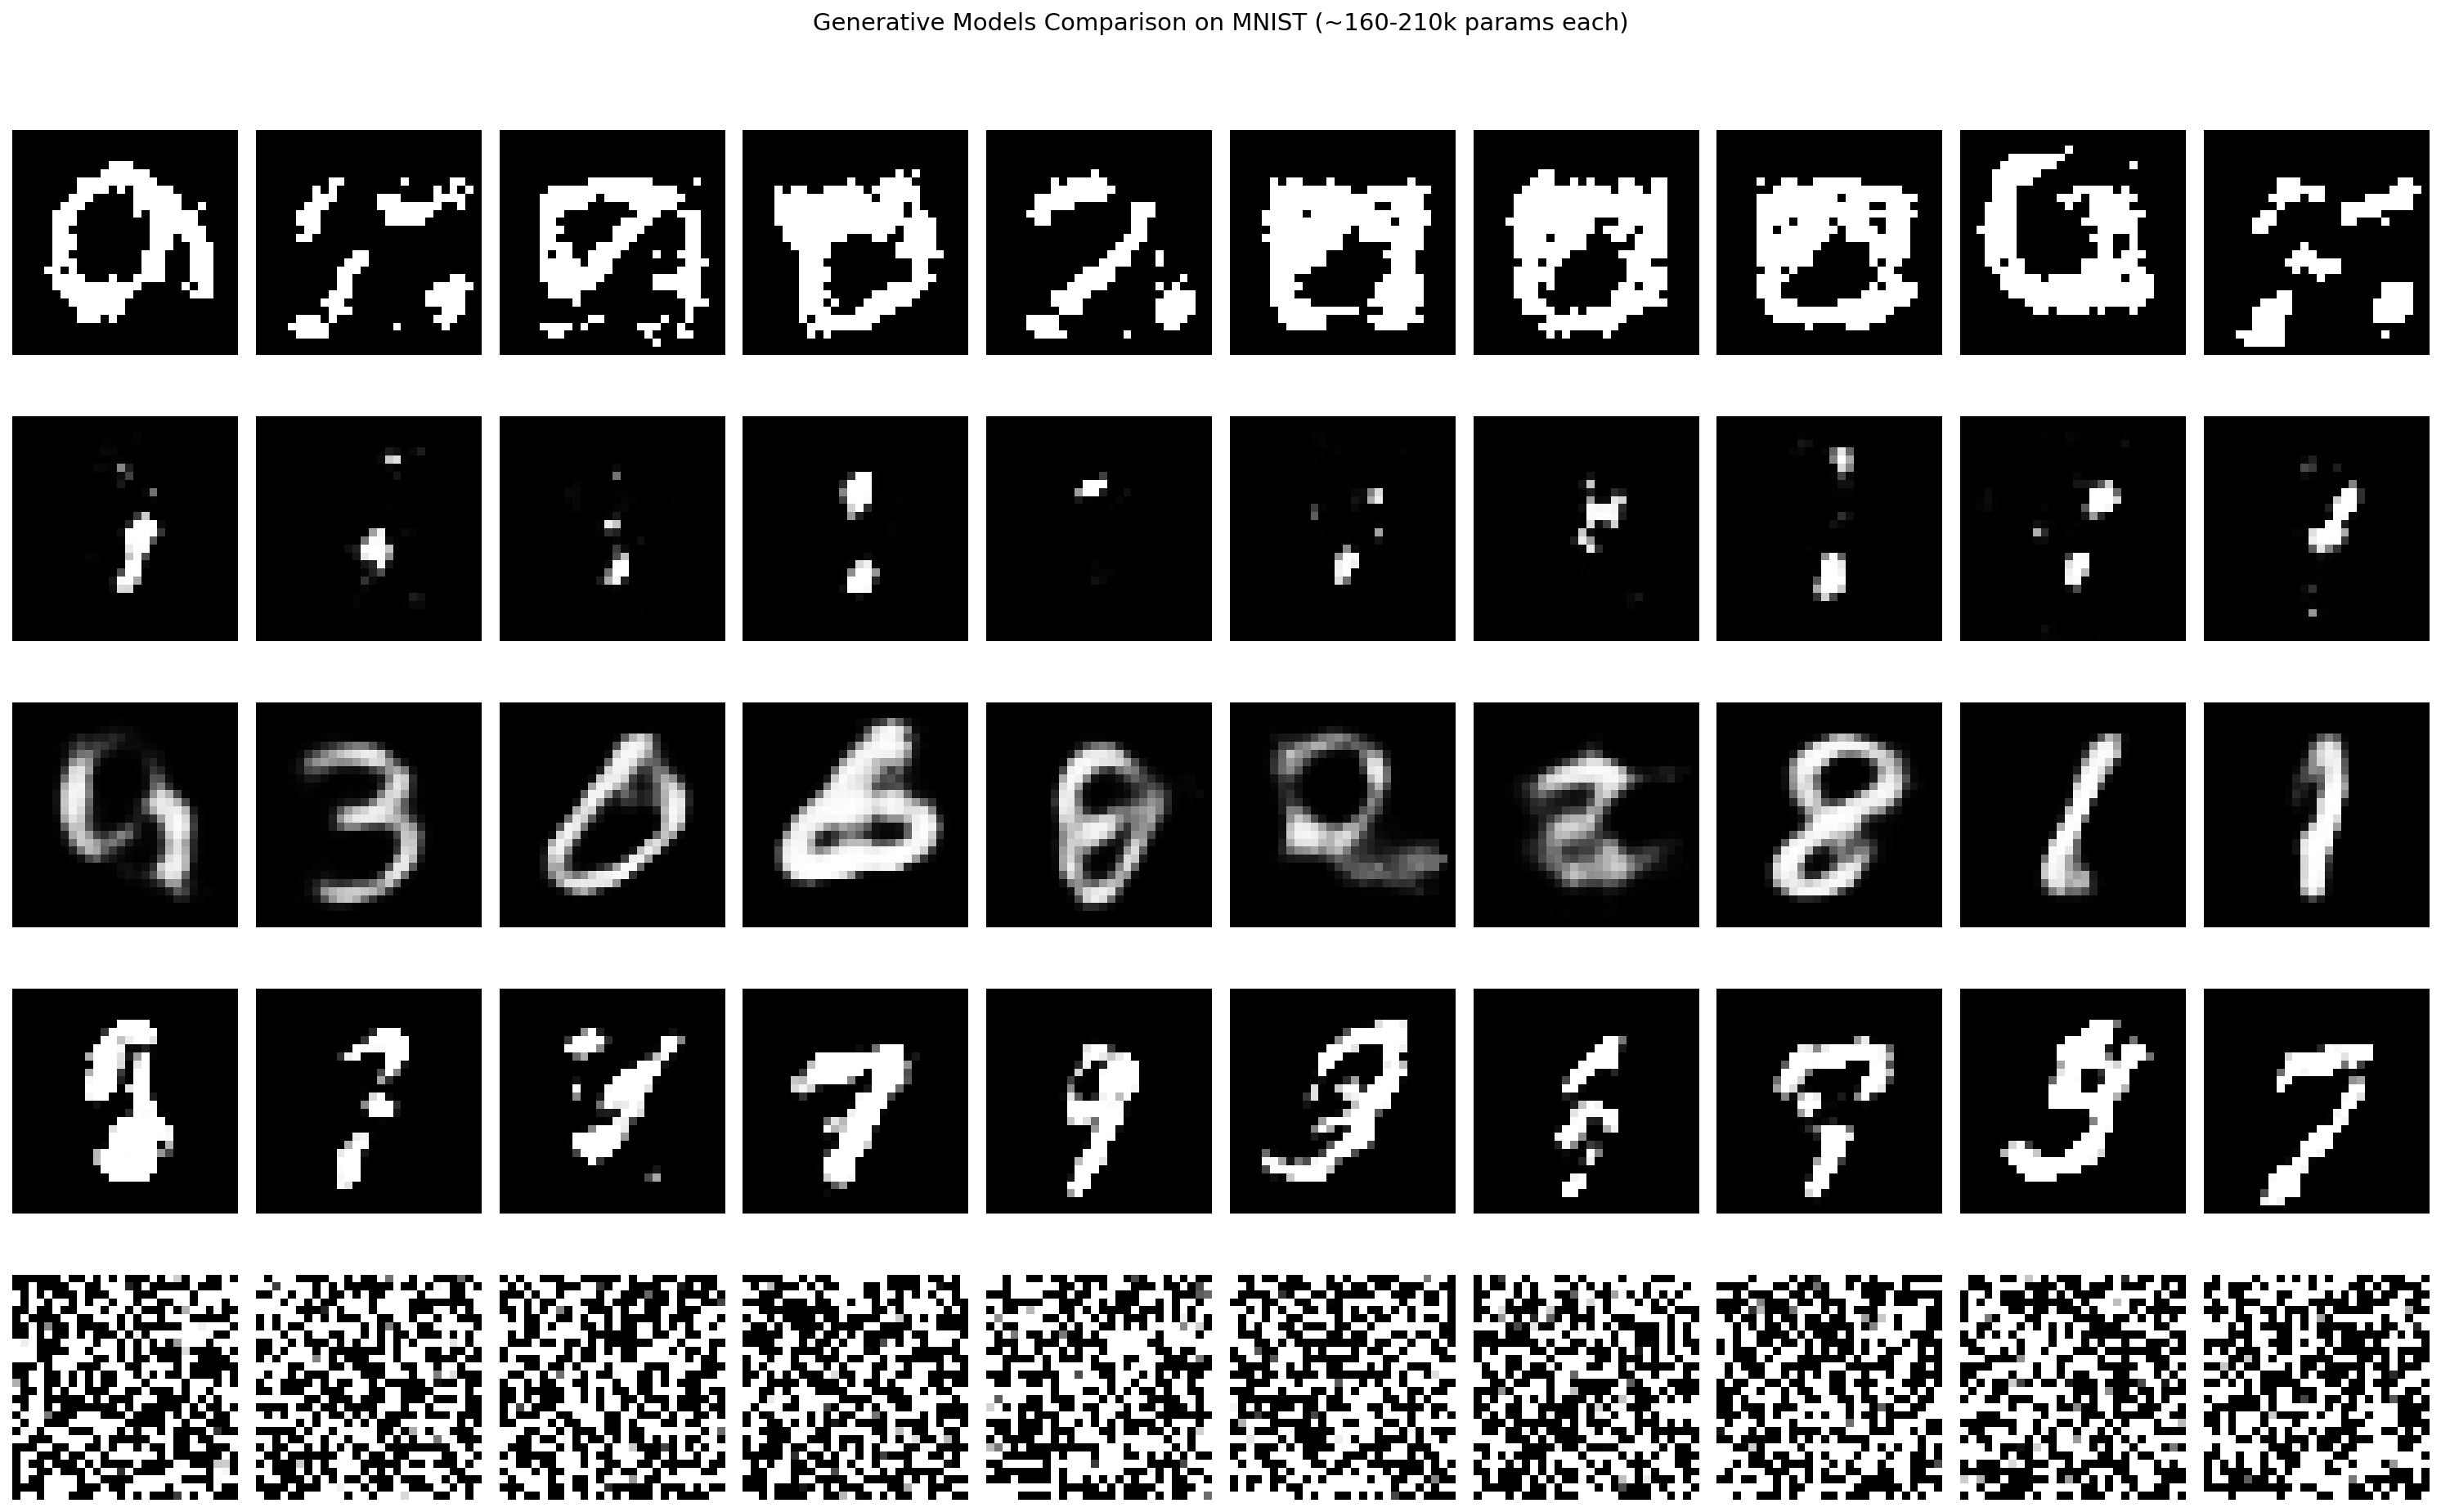
\includegraphics[width=\linewidth]{bonus_comparison.png}
    \caption{Generated MNIST samples from five generative models with approximately the same parameter budget. Generated via the Colab notebook \texttt{notebooks/bonus\_comparison.ipynb}.}
    \label{fig:bonus}
\end{figure}
\noindent\textit{Note: This figure is generated by running the Colab notebook, which downloads MNIST and trains all five models with GPU acceleration.}

\textbf{Analysis.}
\begin{itemize}
    \item The \textbf{RBM} and \textbf{DBN} produce recognizable but noisy binary-looking digits, consistent with their binary stochastic nature.
    \item The \textbf{VAE} generates smooth, plausible digits with good diversity, benefiting from the continuous latent space and the reconstruction + KL objective.
    \item The \textbf{GAN} produces the sharpest images overall, as adversarial training directly optimizes for realism. However, mode collapse can sometimes reduce diversity.
    \item The \textbf{DDPM} produces reasonable but less sharp digits. This is a known limitation of using a simple MLP architecture for denoising: the standard DDPM relies on U-Net architectures with spatial convolutions and attention mechanisms, which cannot be replicated within the $\sim$160k parameter budget. The MLP struggles to denoise 784-dimensional vectors effectively compared to convolutional architectures that exploit spatial structure.
\end{itemize}

This comparison illustrates the trade-off between model families: RBMs/DBNs are simple and principled but limited in output quality; VAEs provide a good balance of quality and training stability; GANs excel at sharpness but are harder to train; and diffusion models require specialized architectures to reach their full potential.

% ============================================================
\section{Conclusion}
% ============================================================

This project demonstrated the complete pipeline from unsupervised feature learning with RBMs to supervised classification with DNNs on MNIST. The key findings are:

\begin{enumerate}
    \item \textbf{Pre-training mitigates the vanishing gradient problem} in deep networks, enabling effective training of architectures with 4--5 hidden layers that would otherwise fail with random initialization.
    \item \textbf{For shallow networks (2 layers), the benefit of pre-training is marginal} when sufficient labeled data is available, but becomes significant in the low-data regime.
    \item \textbf{Pre-trained networks scale better with width}: increasing hidden units to 700 yields consistent improvement for pre-trained networks, while randomly initialized networks plateau earlier.
    \item The \textbf{optimal configuration} for MNIST classification is $[784, 700, 700, 10]$ with pre-training, achieving $2.51\%$ test error.
    \item Among generative models with comparable parameter budgets, \textbf{GANs produce the sharpest samples}, \textbf{VAEs offer the best quality-stability trade-off}, and \textbf{diffusion models require convolutional architectures} to reach their potential.
\end{enumerate}

All code is implemented from scratch in NumPy (core) and PyTorch (bonus only), organized in a modular \texttt{src/} package with reproducible experiment scripts in \texttt{experiments/}.

\end{document}
